\section{Auswertung}
\label{sec:Auswertung}
  \subsection{Winkelrichtgröße}
  Die gemessene Kraft in Abhängigkeit vom dem Auslenkungswinkel wird in der Tabelle \ref{tab:tabelle1} dargestellt.
  Mit der Formel \ref{eqn:D2} wird D berechnet.
  Mithilfe der gemessen Werte für $F$ und $\varphi$ kann mit $r = 20 \, \unit{\centi\meter}$ nun D bestimmt werden.
  Die einzelnen Werte von D sind ebenfalls in \ref{tab:tabelle1} eingetragen. 
  Mit 
  \begin{equation}
    \bar{A} = \frac{1}{n} \sum_{i = 1}^{n} a_i
    \label{eqn:MW}
  \end{equation} 
  wird nun das arithmetische Mittel gebildet. 
  Einsetzen der Werte für D und $n = 11$ ergibt $\bar{D} = 0.02 \, \unit{\newton\meter}$.
  Der Fehler von D ist
  \begin{equation}
     \increment\bar{x}=\sqrt{\frac{1}{\symup{n}\cdot(\symup{n}-1)}(\sum_{i=1}^{\symup{n}} (x_i - \bar{x})^2)}
     \label{eqn:MWfehler}
  \end{equation}.
  Also ergibt sich $\bar{D}=\qty{0,02(0,00168)}{\newton\meter}$.

  \begin{table}[H]
    \centering
    \caption{Kraft in Abhängigkeit zum Auslenkungswinkel}
    \label{tab:tabelle1}
    \sisetup{table-format=1.2}
    \begin{tblr}{
       %% colspec = {S[table-format=3.0] S[table-format=2.1] S},
       colspec={S[table-format=1.3] S[table-format=2.0] S[table-format=1.3]},
        row{1} = {guard, mode=math},
      %%  vline{4} = {2}{-}{text=\clap{$\pm$}},
      }
      \toprule
      F \mathbin{/} \unit{\newton} & \varphi \mathbin{/} \unit{\degree} & \SetCell[c=2]{c} \symbf{D} \mathbin{/} \unit{\newton\meter} & \\
      \midrule
      0.016 &  20 & 0.009\\
      0.046 &  30 & 0.018\\
      0.066 &  40 & 0.019\\
      0.089 &  50 & 0.020\\ 
      0.110  &  60 & 0.021\\
      0.134 &  70 & 0.022\\
      0.162 &  80 & 0.023\\
      0.176 &  90 & 0.022\\
      0.180  & 100 & 0.021\\
      0.200   & 110 & 0.021\\
      0.230  & 120 & 0.022\\
      \bottomrule
    \end{tblr}
  \end{table}
    %% Siehe \autoref{fig:plot} und \autoref{tab:tabelle}!

  
  \subsection{Eigenträgheitsmoment}
  In Tabelle \ref{tab:tabelle2} wird das quadrat des Abstandes der Gewichte von der Drehachse zu dem Quadrat der Schwingungsdauer aufgetragen.

  \begin{table}[H]
    \centering
    \caption{Die Werte des Quadrates der Schwingungsdauer sind in Abhängigkeit zum Quadrat des Abstandes aufgezählt.}
    \label{tab:tabelle2}
    \sisetup{table-format=1.2}
    \begin{tblr}{
        colspec={S[table-format=2.1] S[table-format=2.2]},
        row{1}={guard, mode=math},
        }
        \toprule
        a^2 \mathbin{/} \unit{\centi\meter\squared} & T^2c\mathbin{/} \unit{\second\squared} \\ 
        \midrule     
        2.5  & 12.75\\
        5.0    & 13.84\\
        7.5  & 15.69\\
        10.0   & 18.03\\
        15.0   & 23.54\\
        20.0   & 29.81\\
        22.5 & 32.53\\
        25.0   & 35.84\\
        27.5 & 38.87\\
        30.0   & 41.81\\
        \bottomrule
    \end{tblr}
  \end{table}

  \noindent Um das Trägheitsmoment zu bestimmen wird mit der Formel \ref{eqn:Schwingungsdauer},
  wobei das Trägheitsmoment sich hier aus dem Trägheitsmoment der Massen $I_m$ und der Feder $I_D$ zusammensetzt. Es gilt
  \begin{equation*}
    I=2I_m+I_D
  \end{equation*}
  $I_m$ wird bestimmt mithilfe von \ref{eqn:Trägheit_Zyl_2}, wobei noch beachtet werden muss, dass die Massen den Abstand $a$ 
  von der Drehachse besitzen. Also gilt mit dem Satz von Steiner \ref{eqn:Steiner}, dass
  \begin{equation*}
    I_m=\symup{m} (\frac{\symup{R}^2}{4}+\frac{\symup{h}^2}{12}+a^2)
  \end{equation*}
  In \ref{eqn:Schwingungsdauer} eingesetzt ergibt sich dann die Beziehung
  \begin{equation*}
    T^2=\frac{4\symup{\pi}^2}{\symup{D}}I_D+\frac{m\pi^2}{\symup{D}} (2\symup{R}^2+\frac{2}{3}h^2+8a^2)
  \end{equation*} 
  oder
  \begin{equation}
    T^2=\frac{8\symup{m}\symup{\pi}^2}{\symup{D}}a^2+\frac{\symup{\pi}^2}{\symup{D}}(4I_D+2\symup{m}\symup{R}^2+\frac{2}{3}\symup{m}\symup{h}^2)
    \label{eqn:Eigenschwing}
  \end{equation} 
    \begin{figure}[H]
    \centering
    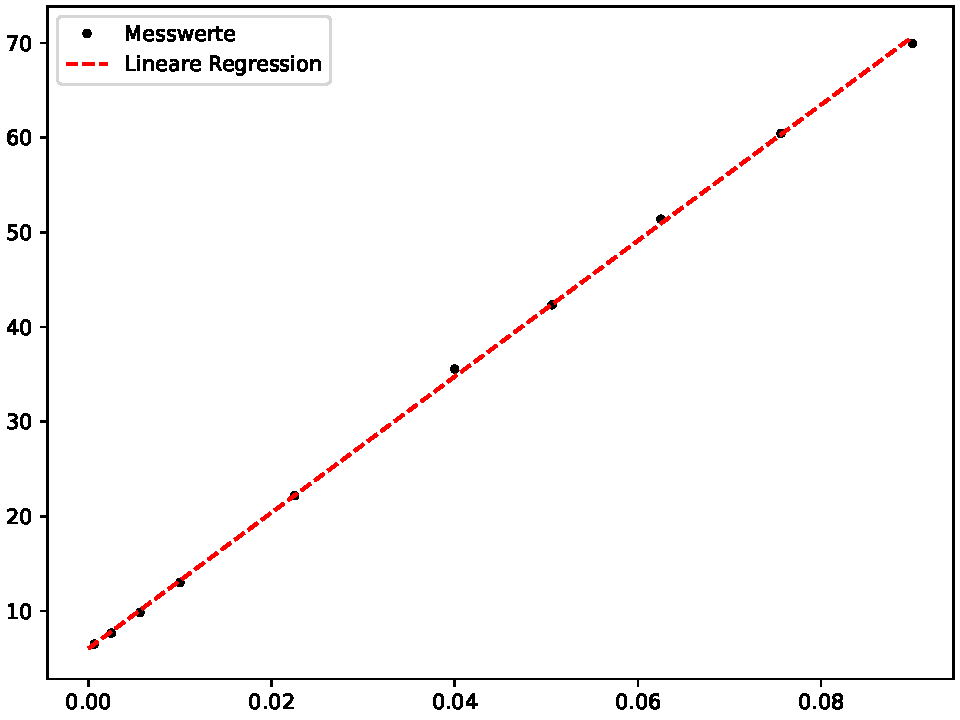
\includegraphics[width=\textwidth]{plot.pdf}
    \caption{lineare Regression von $T^2$ abhängig von $a^2$ }
    \label{fig:plot}
  \end{figure}
  \noindent In Abb\ref{fig:plot} wird $T^2$ zu $a^2$ aufgetragen. Die Steigung der Regressionsgerade beträgt dabei 
  $\qty{717,69(4.45)}{\second\squared \per \meter\squared}$ und der $\symup{T}^2$-Achsenabschnitt $b$ beträgt $\qty{6,04(0.21)}{\second\squared}$.
  %Entsprechend lässt sich ablesen, dass sich das Eigenträgheitsmoment ausdrücken lässt als
  Aus Formel \ref{eqn:Eigenschwing} lässt sich ablesen, dass
  \begin{equation}
    b=\frac{\symup{\pi}^2}{\symup{D}}(4I_D+2\symup{m}\symup{R}^2+\frac{2}{3}\symup{m}\symup{h}^2)
  \end{equation}
  Nach $I_D$ umgeformt ergibt sich dann
  \begin{equation}
    I_D=\frac{\symup{D}\cdot b}{4\symup{\pi}^2}-\frac{1}{2}\symup{m}\symup{R}^2-\frac{1}{6}\symup{m}\symup{h}^2 \text{.}
    \label{eqn:Eigenträgheitsmoment}
  \end{equation}
  
  \noindent Die Höhe der Zylinder beträgt dabei $\qty{2}{\centi\meter}$, der Radius $\qty{4,32}{\centi\meter}$ und die Masse $\qty{261}{\gram}$.
  Entsprechend ergibt sich für das Eigenträgheitsmoment mit 
  \begin{equation}
     \increment f=\sqrt{\sum_{i=1}^{\symup{n}} (\frac{\partial f}{\partial x_i})^2 (\increment x_i)^2}
     \label{eqn:gauß}
  \end{equation}
  
  ein Wert von $\qty{0.003(0.0002)}{\kilo\gram\meter\squared}$.

  \subsection{Trägheitsmomente von Kugel und Zylinder}

  %\begin{table}
  %  \centering
  %  \caption{Schwingungsdauern der Figuren mit einer Auslenkung von 90°}
  %  \label{tab:tabelle4}
  %  \begin{minipage}{0.2\linewidth}
  %  \begin{tblr}{
  %    colspec={S[table-format=1.0] S[table-format=1.2]},
  %    row{1}={guard, mode=math},
  %    }
  %    \toprule
  %      n & 5T  [\unit{\second}] \\
  %    \midrule
  %    1 & 9.12  \\  
  %    2 & 9.37  \\
  %    3 & 9.37  \\
  %    4 & 9.35  \\
  %    5 & 9.41  \\
  %    \bottomrule
  %  \end{tblr}
  %  
  %\end{minipage}
  %\begin{minipage}{0.2\linewidth}
  %  \begin{tblr}{
  %    colspec={S[table-format=1.0] S[table-format=1.2]},
  %    row{1}={guard, mode=math},
  %    }
  %    \toprule
  %    n & 5T[\unit{\second}] \\ 
  %    \midrule
  %    1 & 9.22  \\
  %    2 & 9.32  \\
  %    3 & 9.50  \\
  %    4 & 9.15  \\
  %    5 & 9.22  \\
  %    \bottomrule
  %  \end{tblr}
 %
  %\end{minipage}
  %\end{table}
 
  \begin{table}[H]
   \centering
   \caption{Schwingungsdauern der Körper mit einer Auslenkung von 90°}
   \label{tab:tabelle4}
   \begin{tblr}{
     colspec={S[table-format=1.0] S[table-format=1.2] S[table-format=1.2]},
     row{1}={guard, mode=math},
     }
     \toprule
       n & 5T_K \mathbin{/} \unit{\second} & 5T_Z \mathbin{/} \unit{\second}  \\
     \midrule
     1 & 9.12  & 9.22\\  
     2 & 9.37  & 9.32  \\
     3 & 9.37  & 9.50 \\
     4 & 9.35  & 9.15\\
     5 & 9.41  & 9.22\\
     \bottomrule
   \end{tblr}
  \end{table}
  
  Die Mittlere Periodendauer der Kugel, mit den Werten aus \ref{tab:tabelle4} beträgt hier $\qty{9.324(0.052)}{\second}$ und die des Zylinders $\qty{9.282(0.265)}{\second}$.
 % Mithilfe von den Gleichungn \ref{eqn:Schwingungsdauer} und \ref{eqn:Eigenträgheitsmoment} 
 % beträgt das Trägheitsmoment der Kugel $\qty{0.041(0.008)}{\kilo\gram\meter\squared}$ und das des
 % Zylinders $\qty{0.041(0.002)}{\kilo\gram\meter\squared}$.
  Daraus wird mithilfe von Gleichung \ref{eqn:Schwingungsdauer} das Trägheitsmoment der jeweiligen Objekte berechnet und mit Gleichung \ref{eqn:gauß} der jeweilige Fehler.
  Für die Kugel ergibt damit sich ein Trägheismoment von $I_{e,K}=\qty{-1.24(0.21)e-3}{\kilo\gram\meter\squared}$ und für den
  Zylinder ist $I_{e,Z}=\qty{-1.24(0.25)e-3}{\kilo\gram\meter\squared}$. Hier wurde zu dessen Berechnung das Eigenträgheitsmoment
  bereits abgezogen von den aus Formel \ref{eqn:Schwingungsdauer} resultierenden Trägheismomenten.\\
  Der theoretische Wert für das Trägheitsmoment der Kugel beträgt nach Gleichung \ref{eqn:Trägheit_Kugel} $I_{t,K}=\qty{3e-3}{\kilo\gram\meter\squared}$
  und der des Zylinders nach Gleichung \ref{eqn:Trägheit_Zyl_1} $I_{t,Z}=\qty{3e-3}{\kilo\gram\meter\squared}$.
  
  \subsection{Trägheitsmoment der Puppe}
    \subsubsection{experimentelle Bestimmung von Stellung 1}
    Um das Trägheismoment zu bestimmen wurden 5 Werte mit einem Auslenkungswinkel von $\varphi=90°$ und 5 mit $\varphi=120°$ aufgenommen.
    Diese Werte sind in Tabelle \ref{tab:tabelle5} eingetragen.

   % \begin{table}
   %   \centering
   %   \caption{Schwingungsdauern der Puppe in Stellung 1 mit einer Auslenkung von 90° / 120°}
   %   \label{tab:tabelle5}
   %   \begin{minipage}{0.2\linewidth}
   %   \begin{tblr}{
   %     colspec={S[table-format=1.0] S[table-format=1.2]},
   %     row{1}={guard, mode=math},
   %     }
   %     \toprule
   %       n & 5T [\unit{\second}] \\
   %     \midrule
   %     1 & 3  \\  
   %     2 & 2.9  \\
   %     3 & 2.87  \\
   %     4 & 2.9  \\
   %     5 & 2.97  \\
   %     \bottomrule
   %   \end{tblr}
   %   
   % \end{minipage}
   % \begin{minipage}{0.2\linewidth}
   %   \begin{tblr}{
   %     colspec={S[table-format=1.0] S[table-format=1.2]},
   %     row{1}={guard, mode=math},
   %     }
   %     \toprule
   %     n & 5T[\unit{\second}] \\ 
   %     \midrule
   %     1 & 2.78 \\
   %     2 & 3 \\
   %     3 & 2.94 \\
   %     4 & 3.18  \\
   %     5 & 3.07  \\
   %     \bottomrule
   %   \end{tblr}
   %
   % \end{minipage}
   % \end{table}

   
   \begin{table}[H]
    \centering
    \caption{Schwingungsdauern der Puppe in Stellung 1 mit einer Auslenkung von 90° / 120°}
    \label{tab:tabelle5}
    \begin{tblr}{
      colspec={S[table-format=1.0] S[table-format=1.2] S[table-format=1.2]},
      row{1}={guard, mode=math},
      }
      \toprule
        n & 5T_{90} \mathbin{/} [\unit{\second}] & 5T_{120} \mathbin{/} [\unit{\second}] \\
      \midrule
      1 & 3.00    & 2.78\\  
      2 & 2.90  & 3.00\\
      3 & 2.87 &  2.94\\
      4 & 2.90  & 3.18\\
      5 & 2.97 & 3.07 \\
      \bottomrule
    \end{tblr}
  \end{table}

    Die Mittlere Periodendauer ist $5T=\qty{2.961(0.03)}{\second}$ 
    Durch die Gleichungen \ref{eqn:Schwingungsdauer} und \ref{eqn:Eigenträgheitsmoment} lässt sich, wie bei Kugel und Zylinder, das Trägheitsmoment berechnen.
    Dieses beträgt also mit $I_{e,1}=\qty{1.78(0.01)e-4}{\kilo\gram\meter\squared}$ ergibt sich nach Abzug vom Eigenträgheitsmoment
    $I_{e,1,ges}=\qty{-29.82(0.20)e-3}{\kilo\gram\meter\squared}$.



    \subsubsection{experimentelle Bestimmung von Stellung 2}
    Die in der zweiten Stelling bestimmten Werte sind in Tabelle \ref{tab:tabelle6} aufgelistet.
   % \begin{table}
   %   \centering
   %   \caption{Schwingungsdauern der Puppe in Stellung 2 mit einer Auslenkung von 90° / 120°}
   %   \label{tab:tabelle6}
   %   \begin{minipage}{0.2\linewidth}
   %   \begin{tblr}{
   %     colspec={S[table-format=1.0] S[table-format=1.2]},
   %     row{1}={guard, mode=math},
   %     }
   %     \toprule
   %       n & 5T [\unit{\second}] \\
   %     \midrule
   %     1 & 4  \\  
   %     2 & 4.1  \\
   %     3 & 4  \\
   %     4 & 4.16  \\
   %     5 & 3.94  \\
   %     \bottomrule
   %   \end{tblr}
   %   
   % \end{minipage}
   % \begin{minipage}{0.2\linewidth}
   %   \begin{tblr}{
   %     colspec={S[table-format=1.0] S[table-format=1.2]},
   %     row{1}={guard, mode=math},
   %     }
   %     \toprule
   %     n & 5T[\unit{\second}] \\ 
   %     \midrule
   %     1 & 3.97 \\
   %     2 & 3.94 \\
   %     3 & 3.93 \\
   %     4 & 4.06  \\
   %     5 & 4.13  \\
   %     \bottomrule
   %   \end{tblr}
   %
   % \end{minipage}
   % \end{table}

   \begin{table}[H]
    \centering
    \caption{Schwingungsdauern der Puppe in Stellung 2 mit einer Auslenkung von 90° / 120°}
    \label{tab:tabelle6}
    \begin{tblr}{
      colspec={S[table-format=1.0] S[table-format=1.2] S[table-format=1.2]},
      row{1}={guard, mode=math},
      }
      \toprule
        n & {5T_90} \mathbin{/} [\unit{\second}] & 5T_{120} \mathbin{/} [\unit{\second}] \\
      \midrule
      1 & 4.00    & 3.97\\  
      2 & 4.10  & 3.94\\
      3 & 4.00 &  3.93\\
      4 & 4.16  & 4.06\\
      5 & 3.94 & 4.13 \\
      \bottomrule
    \end{tblr}
  \end{table}

    Die Mittlere Periodendauer ist $5T=\qty{4.023(0.027)}{seconds}$ 
    Analog zu Stellung 1 kann $I_2$ berechnet werden.
    Demnach gilt $I_{e,2}=\qty{3.28(0.17)e-4}{\kilo\gram\meter\squared}$
    und, nach Abzug des Eigenträgheitsmomentes, $I_{e,2,ges}=\qty{-29.67(0.2)e-3}{\kilo\gram\meter\squared}$.

    \subsubsection{Theoretische Berechnung des Trägheismomentes}
    Um das Trägheitsmoment der Puppe zu berechnen wurden der Kopf, der Oberkörper und die einzelnen Arme und Beine als Zylinder genähert.
    Dabei wurde die Höhe der Zylinder einmal abgemessen. 
    Der Durchmesser wurde beim Kopf über 5 und bei den anderen Körperteilen über 10, an verschiedenen Stellen gemessenen, Werte gemittelt.
    Für die Höhen wurden folgende Werte gemessen: \\
    $h_K=\qty{49.9}{\milli\meter}$\quad \
    $h_O=\qty{100.9}{\milli\meter}$\\
    $h_A=\qty{130.3}{\milli\meter}$\quad
    $h_B=\qty{148.6}{\milli\meter}$\\
    Die Werte der Durchmesser sind in der Tabelle \ref{tab:tabelle3} aufgeführt.
    \begin{table}[H]
      \centering
      \caption{Durchmesser der Zylinder der Puppe}
      \label{tab:tabelle3}
      \sisetup{table-format=1.2}
      \begin{tblr}{
          colspec={S S S S[table-format=2.2]},
          row{1}={guard, mode=math},
          }
          \toprule
          d_K \mathbin{/} \unit{\milli\meter} & d_O \mathbin{/} \unit{\milli\meter} & d_A \mathbin{/} \unit{\milli\meter} & d_B \mathbin{/} \unit{\milli\meter}\\
          \midrule     
          26.9 & 40.9 & 15   & 15.8 \\
          27.95& 37.7 & 12.8 & 18.9 \\
          24.8 & 25.8 & 15.7 & 16.5 \\
          21.7 & 31.2 & 13.3 & 15.7 \\
          11.6 & 38.6 & 11.8 & 12 \\
               & 33.1 & 14.4 & 16.9 \\
               & 42.0   & 15.1 & 15.2 \\
               & 26.0   & 12.6 & 13.2 \\
               & 33.3 & 10.1 & 9.3 \\
               & 31.9 & 13.9 & 14.8 \\
          \bottomrule
      \end{tblr}
    \end{table}

    Mit Formel \ref{eqn:MW} wurden dann Werte für die Durchmesser bestimmt und durch 2 geteilt, um den Radius zu erhalten:\\
    $R_K=\qty{11.3(2.01)}{\milli\meter}$ \quad
    $R_O=\qty{17.01(0.90)}{\milli\meter}$\\
    $R_A=\qty{6.23(0.27)}{\milli\meter}$ \quad
    $R_B=\qty{7.12(0.43)}{\milli\meter}$\\

    Für die Berechnung der Trägheismomente sind die Massen der einzelnen Körperteile notwendig.
    Dafür wurde mit einer Waage zuerst die Gesamtmasse der Puppe gemessen: $m_{ges}=\qty{169.3}{\gram}$
    Für die Massen der einzelnen Körperteile wurden dann die Annahme getroffen, dass die Massenverteilung in der Puppe vollständig homogen ist.
    Mithilfe dieser Annahme können die Teilmassen, mit dem Anteil des jeweiligen Volumens an dem des gesamten Körpers, berechnet werden.
    Für die Volumina gilt mit 
    \begin{equation}
      V=\pi r^2 \cdot h
      \label{eqn:volumen}
    \end{equation}
    $V_{ges}=\qty{151.29(2.34)}{\centi\meter\squared}$\\
    $V_K=\qty{20(0.63)}{\centi\meter\squared}$ Anteil am Gesamtvolumen: $\qty{13.23}{\percent}$\\
    $V_O=\qty{91.72(0.26)}{\centi\meter\squared}$ Anteil am Gesamtvolumen: $\qty{60.62}{\percent}$\\
    $V_A=\qty{15.89(0.03)}{\centi\meter\squared}$ Anteil am Gesamtvolumen: $\qty{10.5}{\percent}$\\
    $V_B=\qty{23.67(0.1)}{\centi\meter\squared}$ Anteil am Gesamtvolumen: $\qty{15.64}{\percent}$\\

    Für die einzelnen Massen gilt damit durch 
    \begin{equation}
      m_i=m_{ges} \frac{V_i}{V_{ges}}
    \end{equation}
    $m_K=\qty{22.4}{\gram}$\\
    $m_O=\qty{102.63}{\gram}$\\
    $m_A=\qty{17.78}{\gram}$\\
    $m_B=\qty{26.48}{\gram}$\\

    \subsubsection{Berechnung des Trägheismomentes für Stellung 1}
    Hier wird die Puppe so aufgestellt, wie in \ref{fig:Stellung1} gezeigt.%% Hier bitte Bild 1 einfügen
    Das Gesamtträgheitsmoment setzt sich aus $I_{t}=I_K+I_O+2I_A+2I_B$ zusammen.
    Nun kann das Trägheitsmoment des Kopfes und des Oberkörpers mit Formel \ref{eqn:Trägheit_Zyl_1} berechnet werden.
    Dadurch ergibt sich:\\
    $I_K=\qty{1.43e-6}{\kilo\gram\meter\squared}$\\
    $I_O=\qty{1.5e-5}{\kilo\gram\meter\squared}$\\
    
    Für das Trägheismoment des Beins muss Formel \ref{eqn:Trägheit_Zyl_1} und der Satz von Steiner angewendet werden, da der  Schwerpunkt des Beines nicht in der Drehachse liegt.
    Daraus folgt $I_B=m_B(\frac{R_B^2}{2}+a_B^2)$.
    Hier entspricht $a_B$ der Entfernung vom Schwerpunkt des Beins zur Drehachse, was in dieser Stellung $a_B=\qty{11.35}{\milli\meter}$ entsrpicht.
    Mit dem Einsetzen aller Werte in die Formel ergibt sich $I_B=\qty{4.11e-6}{\kilo\gram\meter\squared}$.\\

    Bei dem Arm muss Formel \ref{eqn:Trägheit_Zyl_2} und ebenfalls der Satz von Steiner verwendet werden.
    Dabei ergibt sich die Formel $I_A=m_A(\frac{R_A^2}{4}+\frac{h_A^2}{12}+a_A^2)$.
    Hier entspricht mit $a_A=R_O+\frac{h_A}{2}$ \; $a_A=\qty{73.75}{\milli\meter}$.
    Daraus folgt $I_A=\qty{1.09e-4}{\kilo\gram\meter\squared}$.\\
    
    Mit $I_{t}=I_K+I_O+2I_A+2I_B$ folgt $I_{t,1}=\qty{2.43e-4}{\kilo\gram\meter\squared}$ und unter Abzug des Eigenträgheitsmoments
     $I_{t,1,ges}=\qty{-2.76e-3}{\kilo\gram\meter\squared}$.

    \subsubsection{Berechnung des Trägheismomentes für Stellung 2}
    Jetzt wird die Puppe wie in \ref{eqn:Stellung2} aufgestellt.%% Hier bitte Bild 2 einfügen
    Hier kann das Trägheitsmoment des Kopfes und des Oberkörpers völlig analog zu Stellung 1 berechnet werden.
    
    Um das Trägheismoment des Beins zu erhalten, muss Formel \ref{eqn:Trägheit_Zyl_2} benutzt werden und da die Drehachse nicht durch den Schwerpunkt verläuft, muss auch hier der Satz von Steiner angewendet werden.
    Daher gilt $I_B=m_B(\frac{R_B^2}{4}+\frac{h_B^2}{12}+a_B^2)$.
    In dieser Stellung ist $a_B=\sqrt{11.35^2+(\frac{h_B}{2})^2}=\qty{75.16}{\milli\meter}$.
    Nach Einsetzen der Werte ergibt sich $I_B=\qty{1.99e-4}{\kilo\gram\meter\squared}$.\\

    Bei dem Arm kann die Berechnung wieder mit $I_A=m_A(\frac{R_A^2}{4}+\frac{h_A^2}{12}+a_A^2)$ durchgeführt werden.
    $a_A$ wird mit $a_A=\sqrt{(R_0+R_A)^2+(\frac{h_A}{2})^2}=\qty{69.17}{\milli\meter}$.
    Damit entspricht $I_A=\qty{1.04e-4}{\kilo\gram\meter\squared}$.\\
    
    Mit $I_{t}=I_K+I_O+2I_A+2I_B$ folgt $I_{t,2}=\qty{6.22e-4}{\kilo\gram\meter\squared}$.
    Wenn davon $I_D$ abgezogen wird, ergibt sich $I_{t,2,ges}=\qty{-2.34e-3}{\kilo\gram\meter\squared}$.





    
    

    

    
